\documentclass[../Cours.tex]{subfiles}
\begin{document}

\chapitre{Addition et soustraction de nombres relatifs}

\partie{Nombres relatifs et comparaison}

\definition{Un nombre est positif s'il est supérieur ou égal à 0.}
\definition{Un nombre est négatif s'il est inférieur ou égal à 0.}
\remarque{0 est à la fois positif et négatif.}
\definition{L'ensemble des nombres positifs et négatifs forment l'ensemble des nombres relatifs.}
\illustration{
\begin{center}
    \begin{tikzpicture}
        \draw[-Latex] (-7,0) -- (7,0);
        \foreach \x in {-6,-5,...,6} {
            \draw (\x,0.1) -- (\x,-0.1);
            \node[below] at (\x, -0.1) {\x};
        }
    \end{tikzpicture}
\end{center}
}

\definition{La distance à zéro (ou valeur absolue) d'un nombre relatif est la distance (la différence) entre le nombre et 0.}

\illustration{
\begin{center}
    \begin{tikzpicture}
        \draw[-Latex] (-7,0) -- (7,0);
        \foreach \x in {-6,-5,...,6} {
            \draw (\x,0.1) -- (\x,-0.1);
            \node[below] at (\x, -0.1) {\x};
        }
        \draw[rouge, Latex-Latex] (-3,0.5) -- (0,0.5);
        \node[rouge, above] at (-1.5,0.5) {3};
    \end{tikzpicture}
\end{center}
}

\begin{listedexemples}
    \item La distance à zéro de -3 est 3.
    \item La distance à zéro de -7 est 7.
    \item La distance à zéro de +4 est 4.
    \item La distance à zéro de 0 est 0.
\end{listedexemples}

\methode{
\begin{itemize}
    \item Pour comparer deux nombres positifs : le plus grand est celui qui a la plus grande distance à zéro.\\
    \centerline{\hfill $4<7$ \hfill $3 > 1,5$ \hfill}
    \item Pour comparer deux nombres négatifs : le plus grand est celui qui a la plus petite distance à zéro.\\
    \centerline{\hfill $-5<-2$ \hfill $-1,7<-1,2$ \hfill}
    \item Pour comparer deux nombres de signes différents : le plus grand est le nombre positif.\\
    \centerline{\hfill $-2<5$ \hfill $1>-17$ \hfill $1,3>-1,5$ \hfill}
\end{itemize}
}

\partie{Addition et soustraction}
\souspartie{Addition}

\methode{\vspace{-1em}
\begin{itemize}
    \item Si deux nombres sont de même signe, la somme est du même signe et on ajoute les distances à zéro.
    \begin{multicols}{2}
        \begin{itemize}
            \item $(+3)+(+4)=(+7)$
            \item $(-2)+(-5)=(-7)$
            \item $(-5)+(-11)=(-16)$
            \item $(-4)+(-6,2)=(-10,2)$
        \end{itemize}
    \end{multicols}
    \item Si deux nombres sont de signes différents, la somme est du même signe que le nombre ayant la plus grande distance à zéro, et on fait la différence entre les distances à zéro.
    \begin{multicols}{2}
        \begin{itemize}
            \item $(-2)+(+3)=(+1)$
            \item $(+5)+(-8)=(-3)$
            \item $(-1,2)+(+0,8)=(-0,4)$
            \item $(-10,5)+(+11,6)=(+1,1)$
        \end{itemize}
    \end{multicols}
\end{itemize}
}

\souspartie{Soustraction}

\propriete{Soustraire un nombre revient à ajouter son opposé.}
\begin{listedexemples}
    \item[$\longrightarrow$] $(+5)-(+3)=(+5)+(-3)=(+2)$
    \item[$\longrightarrow$] $(-7)-(-3)=(-7)+(+3)=(-4)$
    \item[$\longrightarrow$] $(+5)-(-2)=(+5)+(+2)=(+7)$
\end{listedexemples}

\clearpage
\EXERCICES

\begin{questions}
    \exercice ~~\textsc{Les nombres croisés}\\
    \begin{wrapfigure}{r}{0.4\linewidth}
    \begin{tikzpicture}
        \draw (0,0) grid (4,4);
        \draw[fill=noir] (0,0) rectangle (1,1) (1,1) rectangle (2,2) (2,0) rectangle (3,1) (3,2) rectangle (4,3) (2,3) rectangle (3,4);
    \end{tikzpicture}
    \end{wrapfigure}
    \textbf{Horizontalement :}
    \begin{enumerate}
        \item Opposé de 8 $\blacksquare$ Positif et négatif à la fois
        \item $-13+215-7-6$
        \item Opposé de $-5$ $\blacksquare$ $-(-6-6)$
        \item $-0.5+1.5$ $\blacksquare$ Opposé de l'opposé de $-6$
    \end{enumerate}
    \textbf{Verticalement :}
    \begin{enumerate}
        \item Entier relatif compris entre $-15,6$ et $-14,9$
        \item $(-3+7) - (4-88)$ $\blacksquare$ $(-4) - (-5)$
        \item $52+34 - (35-41) - (8-7)$
        \item $(-3) - (-3)$ $\blacksquare$ 2 dizaines et 6 unités
    \end{enumerate}
    
    \exercice \textsc{Échelles de température}\\
    
    Dans la vie de tous les jours, la température est mesurées en degrés Celcius (°C). Mais il existe une autre échelle de température, l'échelle Kelvin, définie de la manière suivante :
    
    \[ T_{Kelvin} = T_{°Celcius} + \num{273,15} \]
    
    Par exemple, \qty{30}{°C} = \qty{303.15}{K}.
    
        \question Convertir \qty{50}{°C}, \qty{-15}{°C} et \qty{23,67}{°C} en Kelvins
        \question Convertir \qty{350}{K}, \qty{5000}{K} et \qty{25}{K} en degrés Celcius
        \question À quelle température l'eau liquide devient solide ? À quelle température l'eau liquide bouille-t-elle ? Donner les réponses en degrés Celcius et en Kelvins.
        \question Le zéro absolu est la température la plus basse possible dans l'univers, elle correspond à \qty{0}{K}. Donner sa valeur en degrés Celcius.
        
    \exercice ~~\textsc{Carré magique}\\
    
    \begin{wrapfigure}{r}{0.4\linewidth}
    \vspace{-1cm}
    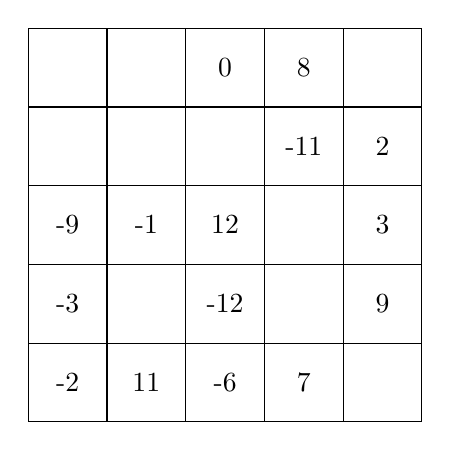
\begin{tikzpicture}
        \draw (1,1) grid (6,6);
        \node at (1.5,1.5) {-2};
        \node at (2.5,1.5) {11};
        \node at (3.5,1.5) {-6};
        \node at (4.5,1.5) {7};
        \node at (1.5,2.5) {-3};
        \node at (3.5,2.5) {-12};
        \node at (5.5,2.5) {9};
        \node at (1.5,3.5) {-9};
        \node at (2.5,3.5) {-1};
        \node at (3.5,3.5) {12};
        \node at (5.5,3.5) {3};
        \node at (4.5,4.5) {-11};
        \node at (5.5,4.5) {2};
        \node at (3.5,5.5) {0};
        \node at (4.5,5.5) {8};
    \end{tikzpicture}
    \end{wrapfigure}
    
    Si on additionne toutes les valeurs d'une ligne, d'une colonne ou d'une diagonale, on obtient 0. Tous les nombres entiers de $-12$ à $12$ sont présents dans le carré.\\
    Complète le carré magique ci-dessous.
    
    \vspace{2cm}
    \exercice ~~\textsc{Histoire antique}
    
    \question Compléter le tableau en remettant dans l'ordre croissant les dates suivantes : \\-356 ; -51 ; -1300 ; -330 ; -218 ; -776
    \question Compléter ensuite la colonne << durée >> en calculant la durée séparant chacun des évènements de l'Histoire antique.
    \begin{center}
    \begin{tabular}{|c|c|c|}\hline
    Évènements & année & durée \\\hline
    Naissance de Ramsès II  & & \\\hline
    $1^{er}$ jeux olympiques antiques  & & \\\hline
    Naissance d'Alexandre le grand & & \\\hline
    Naissance d'Euclide d'Alexandrie & & \\\hline
    Hannibal traverse les Alpes & & \\\hline
    Cléopâtre reine d'Égypte & & \\\hline
    \end{tabular}
    \end{center}
\end{questions}

\end{document}

\newcommand{\figurethales}[6]{
    \begin{tikzpicture}
        \coordinate (A) at (0,0);
        \coordinate (B) at (3,1.5);
        \coordinate (C) at (3,-1.5);
        \coordinate (D) at (6,3);
        \coordinate (E) at (6,-3);
        \draw (A) node[left]{A} -- (D) node[right]{D} -- (E) node[right]{E} --cycle;
        \draw (B) node[above]{B} -- (C) node[below]{C};
        \draw[red,Latex-Latex] ($(A)!0.1!(B)+(0,-0.2)$) -- ($(A)!0.95!(B)+(0,-0.2)$);
        \draw[blue,Latex-Latex] ($(A)!0.1!(C)+(0,0.2)$) -- ($(A)!0.95!(C)+(0,0.2)$);
        \node[red,rotate=30] at ($(A)!0.7!(B)+(0,-0.5)$) {\qty{#1}{\centi\metre}};
        \node[blue,rotate=-30] at ($(A)!0.7!(C)+(0,0.5)$) {\qty{#2}{\centi\metre}};
        \draw[Latex-Latex] ($(A)+(0,0.8)$) -- ($(D)+(0,0.8)$);
        \draw[Latex-Latex] ($(A)+(0,-0.8)$) -- ($(E)+(0,-0.8)$);
        \node[rotate=30] at ($(A)!0.45!(D)+(0,1.15)$) {\qty{#4}{\centi\metre}};
        \node[rotate=-30] at ($(A)!0.45!(E)+(0,-1.15)$) {\qty{#5}{\centi\metre}};
        \draw[Latex-Latex] ($(B)!0.05!(C)+(0.2,0)$) -- ($(B)!0.95!(C)+(0.2,0)$);
        \draw[Latex-Latex] ($(D)!0.05!(E)+(0.2,0)$) -- ($(D)!0.95!(E)+(0.2,0)$);
        \node[anchor=west] at ($(B)!0.5!(C)+(0.15,0)$) {\qty{#3}{\centi\metre}};
        \node[anchor=west] at ($(D)!0.5!(E)+(0.15,0)$) {?};
        \node at (3,4) {\fbox{Figure n°#6}};
    \end{tikzpicture}
}

\figurethales{3}{4}{5}{18}{24}{1}~\figurethales{7}{2}{8}{28}{8}{2}

\figurethales{1}{2}{2.5}{3}{6}{3}~\figurethales{5}{6}{7}{20}{24}{4}

\newcommand{\theoremepythagore}[3]{
    \begin{tikzpicture}[scale=0.8]
        \coordinate (A) at (0,0);
        \coordinate (B) at (3,0);
        \coordinate (C) at (3,4);
        \node at (3,5) {\fbox{Figure n°#3}};
        \draw (A) node[left]{$A$} -- (B) node[right]{$B$} -- (C) node[right]{$C$} -- cycle;
        \node[below] at ($(A)!0.5!(B)$) {\qty{#1}{\centi\metre}};
        \node[right] at ($(B)!0.5!(C)$) {\qty{#2}{\centi\metre}};
        \node[left] at ($(A)!0.5!(C)$) {?};
    \end{tikzpicture}
}

\clearpage
\theoremepythagore{3}{4}{1} \theoremepythagore{2}{6}{2} \theoremepythagore{8}{14}{3} 

\theoremepythagore{2}{8}{4} \theoremepythagore{4.5}{4.5}{5} \theoremepythagore{9}{2}{6}